

\section*{Houdini section}
\markboth{\hspace{1cm}exercices}{Joris Putteneers\hspace{1cm}}



word\footnote{Explanation of the word.} that Addjword\footnote{Explanation of the word.} thatjord\footnote{Explanation of the word.} thatYou can find the source code on GitHub: \url{https://github.com/your-username/your-repository}.


%\keywords{-5}{-4cm}{16cm}{Keyword 1, Keyword 2, Keyword 3Keyword 1, Keyword 2, Keyword 3Keyword 1, Keyword 2, Keyword 3}

P
raesent in sapien. Lorem ipsum dolor sit amet, consectetuer adipiscing elit.
Duis fringilla tristique neque. Sed interdum libero ut metus. Pellentesque
placerat. Nam rutrum augue a leo. Morbi sed elit sit amet ante lobortis
sollicitudin.Praesent in sapien. Lorem ipsum dolor sit amet, consectetuer
adipiscing elit. Duis fringilla tristique neque. Sed interdum libero ut metus.
P

\begin{multicols}{2} % Specify the number of columns
    \lipsum[1] % Your Lorem Ipsum text goes here
 \noindent   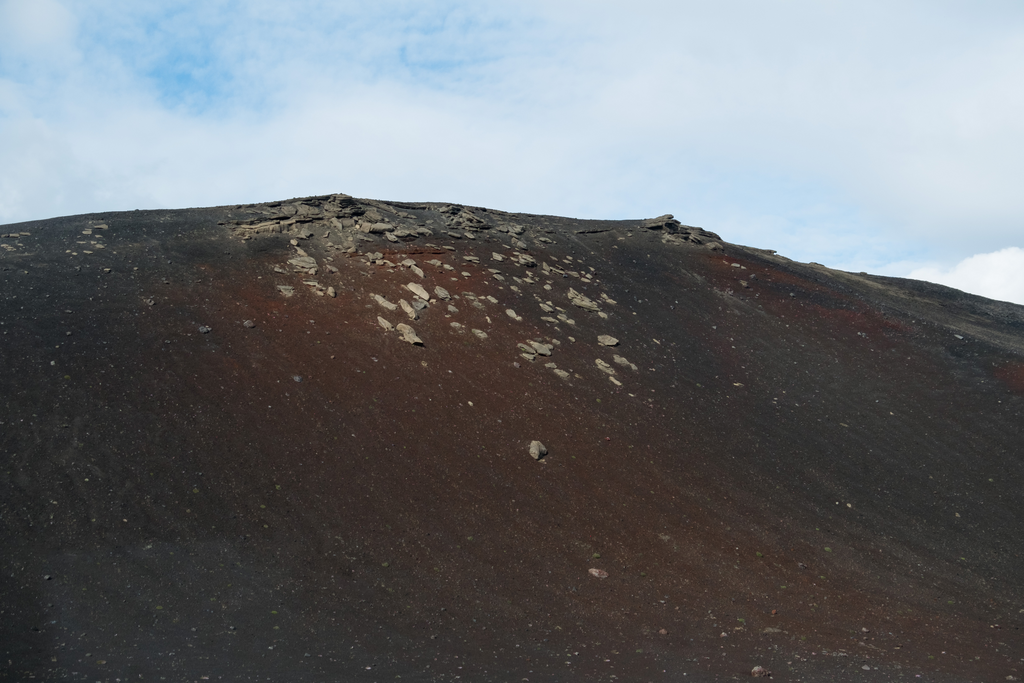
\includegraphics[width=\linewidth]{sections/assignment_1/t.png} % Adjust width as needed
    \lipsum[1-4] % Your Lorem Ipsum text goes here
\end{multicols}

ellentesque placerat. Nam rutrum augue a leo. Morbi sed elit sit amet ante
lobortis sollicitudin. Pellentesque placerat. Nam rutrum augue a leo. Morbi sed
e
Praesent in sapien. Lorem ipsum dolor sit amet, consectetuer adipiscing elit.
Duis fringilla tristique neque. Sed interdum libero ut metus. Pellentesque
placerat. Nam rutrum augue a leo. Morbi sed elit sit amet ante lobortis
sollicitudin.Praesent in sapien. Lorem ipsum dolor sit amet, consectetuer
adipiscing elit. Duis fringilla tristique neque. Sed interdum libero ut metus.
Pellentesque placerat. Nam rutrum augue a leo. Morbi sed elit sit amet ante
lobortis sollicitudin. Pellentesque placerat. Nam rutrum augue a leo. Morbi sed
elit sit amet ante lobortis sollicitudin
%\keywords{-13}{-4cm}{16cm}{Keyword 1, Keyword 2, Keyword 3}









































